
The core calculus of NomosUC relies on \emph{binary session types}~\cite{caires2010session}:
a type discipline for communication-centric programming derived from a Curry-Howard interpretation
of intuitionistic linear logic~\cite{girard1987linear}.
Under this correspondence, a process term $P$ is assigned to
a logical judgment of the form $A_1, \ldots A_n \vdash C$ and each antecedent as well as the succedent is
labeled with a \emph{channel} to obtain
\begin{center}
\begin{minipage}{0cm}
\begin{tabbing}
$(x_1 : A_1), (x_2 : A_2), \ldots, (x_n : A_n) \vdash P :: (z : C)$
\end{tabbing}
\end{minipage}
\end{center}

The resulting judgment states that process $P$ \emph{provides} a service
of session type $C$ along channel $z$, \emph{using} the services of session
types $A_1, \ldots, A_n$ provided along channels $x_1, \ldots, x_n$ respectively.
We mandate all channel names to be distinct for the judgment
to be \emph{well-formed}.
The linear antecedents are often abbreviated to $\D$.

Formally, the typing judgment for processes in NomosUC is written as
\begin{center}
\begin{minipage}{0cm}
\begin{tabbing}
$\Sg \semi k \semi \Tokens \semi \Psi \semi \D \entailpot{q}{q'} P :: (x : A)$
\end{tabbing}
\end{minipage}
\end{center}

$\Sg$ denotes the signature containing type and process definitions and $k$
denotes the security parameter.
Both these quantities are globally known and fixed, therefore we omit them from
most typing rules for brevity.
$\Tokens$ describes the total and current ($=$ received - sent) import tokens
of each type stored in the process (explained more in Section~\ref{sec:import}).
$\Psi$ represents the functional data structures and $\D$ collects the
session-typed channels along with an optional \emph{write token} $\wt$
(to resolve non-determinism in the semantics) used by the process.
Intuitively, the process sending a message \emph{must possess} the write
token which is then transferred to the receiver along with the message.
Globally, the process owning the write token is activated to take the
next execution step.
Finally, $P$ is the process expression that is currently being executed and
the process offers channel $x$ of type $A$.
Similar to import tokens, the natural number annotations $q$ and $q'$ on the turnstile
denote the total and current potential stored in the process.
We will gradually explain each component of the language, initiating
with the basic system of session types.
For simplicity of exposition, we will display the yet unexplained
parts of the system in blue.

The operational semantics for session-typed programs are formalized as a
system of \emph{multiset rewriting rules}~\cite{cervesato2009relating}.
These rules consist of semantic objects $\proc{c}{P}$ and $\msg{c}{M}$ describing
process $P$ (or message $M$) providing service along channel $c$.
Remarkably, in this formulation, a message is just a particular form of process,
thereby not requiring any special rules for typing; it can be typed just as processes.
Since we track computational cost as well in NomosUC, we extend the semantic objects
to $\proc{c}{w, P}$ and $\msg{c}{w, P}$ where work counter $w$ stores the work performed
(number of computational steps executed) by process $P$ (resp. message $M$).

\subsection{Session Type Constructors}
\label{subsec:constructors}

The Curry-Howard correspondence gives each linear logic connective an
interpretation as a session type.
We follow a detailed description of each of these session type constructors,
but restricted to a subset that are sufficient for the applications of NomosUC.

\paragraph*{\textbf{Choice Operators}}
The internal choice $\ichoice{\ell : A_\ell}_{\ell \in L}$ constructor
is an $n$-ary labeled generalization of the additive disjunction $A \oplus B$.
A process that provides $x : \ichoice{\ell : A_\ell}_{\ell \in L}$ can send
any label $k \in L$ along $x$ and then continue by providing $x : A_k$. The
corresponding process is written as $(\esendl{x}{k} \semi P)$, where
$P$ is the continuation that provides $A_k$.
On the other end of the channel, the client branches on the label received along $x$.
The provider and client are typed according to the following $\oplus R$ and $\oplus L$
rules respectively.
\begin{mathpar}
  \infer[{\oplus}R]
  {\B{\Tokens \semi \Psi} \semi \wt, \D \entailpot{\B{q}}{\B{q'}} (\esendl{x}{k} \semi P) ::
    (x : \ichoice{\ell : A_\ell}_{\ell \in L})}
  {(k \in L) \qquad \B{\Tokens \semi \Psi} \semi \D \entailpot{\B{q}}{\B{q'}} P :: (x : A_k)}
\and
  \infer[{\oplus}L]
  {\B{\Tokens \semi \Psi} \semi \D, (x : \ichoice{\ell : A_\ell}_{\ell \in L})
    \entailpot{\B{q}}{\B{q'}} \ecase{x}{\ell}{Q_\ell}_{\ell \in L} :: (z : C)}
  {(\forall \ell \in L) \qquad \B{\Tokens \semi \Psi} \semi \wt, \D, (x : A_\ell)
    \entailpot{\B{q}}{\B{q'}} Q_\ell :: (z : C)}
\end{mathpar}
Additionally, the provider should possess the write token to be able to send the
label $k$. Dually, the client receives the write token with the label to continue
execution.

Operationally, since communication is asynchronous, the process
$(\esendl{c}{k} \semi P)$ sends a message $k$
along $c$ and continues as $P$ without waiting for it to be received.
As a technical device to ensure that consecutive messages on a
channel arrive in order, the sender also creates a fresh continuation
channel $c'$ so that the message $k$ is actually represented as
$(\esendl{c}{k} \semi \fwd{c}{c'})$ (read: send $k$ along $c$ and
continue as $c'$). The provider substitutes $c'$ for $c$ enforcing
that the next message is sent on $c'$.
The work counter of the process remains unaltered, and the new message
is created with work $0$.
\begin{tabbing}
$(\oplus S) : \proc{c}{w, \esendl{c}{k} \semi P} \step \proc{c'}{w, [c'/c]P},$ \\
\quad \qquad $\msg{c}{0, \esendl{c}{k} \semi \fwd{c}{c'}} \qquad \qquad \qquad \qquad \quad \fresh{c'}$
\end{tabbing}
When the message $k$ is received along $c$, the client selects branch
$k$ and also substitutes the continuation channel $c'$ for $c$, thereby
ensuring that it receives the next message on $c'$. This implicit
substitution of the continuation channel ensures the ordering of the
messages.
The client process also collects the work performed by the message, if
there is any.
\begin{tabbing}
$(\oplus C) :$ \= $\msg{c}{w, \esendl{c}{k} \semi \fwd{c}{c'}},
\proc{d}{w', \ecase{c}{\ell}{Q_\ell}}$ \\
$\qquad \qquad \step \proc{d}{w+w',[c'/c]Q_k}$
\end{tabbing}

The dual of internal choice is \emph{external choice} $\echoice{\ell :
A_\ell}_{\ell \in L}$, the $n$-ary labeled generalization of the
additive conjunction $A \with B$. This dual operator simply reverses
the role of the provider and client. The provider process of
$x : \echoice{\ell : A_\ell}_{\ell \in L}$ branches on receiving a label
using the expression $\ecase{x}{\ell}{Q_\ell}_{\ell \in L}$,
while the client sends one such label in $L$ using the expression $(\esendl{x}{k} \semi P)$.
% $k \in L$ (described in $\with R$), while the client sends this label
% (described in $\with L$).
% \begin{mathpar}
%   \footnotesize
%   \infer[\with R]
%   {\B{k \semi \Tokens \semi \Psi} \semi \D \entailpot{\B{q}}{\B{q'}} \ecase{x}{\ell}{P_\ell}_{\ell \in L} ::
%     (x : \echoice{\ell : A_\ell}_{\ell \in L})}
%   {(\forall \ell \in L) \qquad \B{k \semi \Tokens \semi \Psi} \semi \wt, \D
%     \entailpot{\B{q}}{\B{q'}} P_\ell :: (x : A_\ell)}
% \end{mathpar}
% \begin{mathpar}
%   \footnotesize
%   \infer[\with L]
%   {\B{k \semi \Tokens \semi \Psi} \semi \wt, \D, (x : \echoice{\ell : A_\ell}_{\ell \in L})
%     \entailpot{\B{q}}{\B{q'}} \esendl{x}{k} \semi Q :: (z : C)}
%   {\B{k \semi \Tokens \semi \Psi} \semi \D, (x : A_k) \entailpot{\B{q}}{\B{q'}} Q :: (z : C)}
% \end{mathpar}
Dual to internal choice, the client contains the write token which is
sent to the provider along with the label.
The typing and semantics rules for external choice are just the inverse of internal choice,
and presented in Appendix~\ref{app:typing_rules}.

\paragraph*{\textbf{Termination}}
The type $\one$, the multiplicative unit of linear logic, represents
termination of a process, which is not allowed to use
any linear channels. A terminating process offering on $x : \one$ simply
closes channel $x$ using the expression $\eclose{x}$ while the client waits
for this close message to arrive using the expression $\ewait{x} \semi Q$
and then continues executing $Q$.
The typing rules are presented in Appendix~\ref{app:typing_rules}.
% Operationally, the provider converts into a closing message
% with no continuation since the offered channel terminates.
% \begin{tabbing}
% $(\one S) : \proc{c}{\eclose{c}} \step \msg{c}{\eclose{c}}$ \\
% $(\one C) : \msg{c}{\eclose{c}}, \proc{d}{\ewait{c} \semi Q} \step
% \proc{d}{Q}$
% \end{tabbing}

% The provider receives the branching label $k$ sent by the provider. Both
% processes perform appropriate substitutions to ensure the order of messages
% sent and received is preserved.
% \[
% \begin{array}{lll}
% (\with S) & \proc{d}{\esendl{c}{k} \semi Q} \step \msg{c'}{\esendl{c}{k}
% \semi \fwd{c'}{c}}, \proc{d}{[c'/c]Q} & \fresh{c'} \\
% (\with C) & \proc{c}{\ecase{c}{\ell}{Q_\ell}_{\ell \in L}},
% \msg{c'}{\esendl{c}{k} \semi \fwd{c'}{c}} \step \proc{c'}{[c'/c]Q_k}
% \end{array}
% \]

\paragraph*{\textbf{Exchanging Functional Data}}
So far, we have discussed the channels in $\D$ in the typing judgment for NomosUC.
Now, we turn out attention to the functional layer $\Psi$ that contains the
traditional data structures and values.
Communicating a \emph{value} of the functional fragment along a channel
is expressed at the type level by adding the following two session types.
\begin{center}
\begin{minipage}{0cm}
\begin{tabbing}
$A ::= \ldots \mid \tau \arrow A \mid \tau \product A$
\end{tabbing}
\end{minipage}
\end{center}
Here, $\tau$ describes a functional type, e.g. $\m{int}, \m{bool}, \tau \; \m{list}$, etc
(we assume the language contains standard functional types).
The type $\tau \arrow A$ prescribes receiving a value of type $\tau$
with continuation type $A$, while its dual $\tau \product A$ prescribes
sending a value of type $\tau$ with continuation $A$. The corresponding
typing rules for arrow ($\arrow R, \arrow L$) are given in Appendix~\ref{app:typing_rules}.
The $\product$ operator is dual to $\arrow$ reversing the roles of provider and client,
and we omit its explanation for brevity.

\subsection{Shared Session Types and ITM Channels}
\label{subsec:communicators}
%Despite the seemingly structured nature of execution in UC, the framework is meant to
%capture arbitrary connections, communication patterns, or configurations of ITMs.
%However, linear session types can prove to be quite restrictive in terms of realizing
%arbitrary communication patterns in practical cryptographic protocols.
%In this section, we highlight a common communication pattern in UC that requires introducing
%the notion of shared session types~\cite{balzer2017manifest} to be expressible in NomosUC.

Consider two ITMs $P$ and $Q$ that communicate in the following way. If $P$ is activated first,
it sends a message to $Q$ and terminates, but if $Q$ is activated first it writes a message to $P$, 
$P$ writes a message back, and communication terminates.
Session types require it to be statically known which party will write next to a channel so such
a communication pattern can not be realized by juts a single session type.

If we try to resolve this by splitting communication among two channels, we may type them as
%\begin{center}
\vspace{2mm}

{\centering
 $\m{PtoQ} = \ichoice{\mb{one}: int \tensor 1}$ \\
 $\m{QtoP} = \echoice{\mb{one}: int \tensor \ichoice{\mb{end}: int \tensor 1}}$
%\end{center}
\par}
\vspace{2mm}
However, session types naturally impose a \emph{parent-child relationship} among processes by requiring
every channel to have a provider and client endpoint.
Moreover, these endpoints are fixed, i.e., a process cannot transition from being a client of
a channel to its provider, or vice-versa.
If $P$ and $Q$ are connected with channels they offer each other, the provider-client relationship
is undefined as one process must spawn the other.
In general, this restriction results in an acyclic tree-like topology among processes where parents progressively
spawn child processes becoming the client to the channel provided by the child.
%On the other hand, UC places no such restriction on communication and cyclic communication
%is quite common in UC protocols.
Thus, a direct translation from ITM terms to NomosUC expressions can result in cyclic
dependency among channels, thus causing the program to be ill-typed.

% The pattern emerges from the following code: a machine $P$ either writes to another machine $Q$ or is written to by $Q$. 
% At first glance, it is a trivial scenario, but we encounter a problem trying to encode this with a single session type.
% A example are machines $P$ and $Q$ which execute as follows:
% \begin{itemize}
% 	\item An external machines flips a bit and activates either $P$ or $Q$.
% 	\item If $P$ is activated it writes to $Q$ and the execution terminates. 
% 	\item Otherwise, if $Q$ is activated, it writes a message to $P$, $P$ writes something back, and the execution terminates.
% \end{itemize}
% A single type between $P$ and $Q$ would have to allow either of the two parties to write on the channel, but session types require it to be statically known.
%
% If we try to separate communication between $P$ and $Q$ into two uni-directional channel, we can express the session type for each of the channels:
% \begin{center}
% \parbox{0cm}{
% \begin{tabbing}
% $\m{PtoQ} = \ichoice{\mb{``one''}: int \tensor 1}$ \\
% $\m{QtoP} = \echoice{\mb{``one''}: int \tensor \ichoice{\mb{``end''}: int \tensor 1}}$
% \end{tabbing}}
% \end{center}
%
% This approach, however, poses another problem. 
% Channels are only created by a process offering them, and a process can only offer a single channel.
% Without adding any additional processes, $P$ must offer a channel to $Q$ and $Q$ offer one to $P$. 
% Each of them becomes both a provider and a client to the other, and provider/client ambiguity is not allowed in Nomos. 
% Logically, one process must have spawned the other, and such a cycle would be impossible to realize.

To enable arbitrary communication between two processes without forcing a parent-child relationship, we introduce
the concept of \emph{providerless channels} using \emph{communicator processes} that rely on recently introduced shared session types~\cite{balzer2017manifest}.
Communicators act as a buffer between two processes allowing them to exchange messages via the communicator.
Communicators also break the parent-child relationship by offering a \emph{shared channel that can have multiple clients}
(unlike linear channels that can have only one client) that is then used by both the sender and receiver processes.

The communicator has the following polymorphic type:
%\begin{center}

\vspace{-1mm}
{\centering
\parbox{0cm}{
\begin{tabbing}
$\m{comm[\tau]} = \up \echoice{$\=$\mb{send}: \m{\tau} \arrow \m \down \m{comm[\tau]},$\\
\>$\mb{recv}: \ichoice{$\=$\mb{yes}: \m{\tau} \;\product \down \m{comm[\tau]},
\mb{no}: \; \down \m{comm[\tau]}}}$
\end{tabbing}}
%\end{center}
\par}


The communicator type relies on shared type constructors $\up$ and $\down$.
The type initiates with an $\up$ indicating that the communicator channel must be \emph{acquired} to interact with it.
Because the channel has two clients (the sender and the receiver), either of them can send this acquire request.
Once acquired, the sender uses the $\mb{SEND}$ branch of the type while the receiver interacts with the $\mb{RECV}$ branch.
In the former case, the communicator receives the $\mb{SEND}$ message from the sender followed by the actual
message of type $\tau$ as indicated by the $\arrow$ constructor.
Then the sender releases the channel so that the receiver can interact with the communicator and check, with $\mb{RECV}$ whether 
there is a message waiting or not.
We provide the full typing rule of shared session types in Appendix~\ref{app:typing_rules}.
%Then, the type transitions to $\down$ meaning that the sender sends a \emph{release} request to the communicator effectively
%detaching from it so that the receiver can interact with the communicator.
%In the latter case, the communicator gets the $\mb{RECV}$ request from the receiver and checks whether the there is a message
%waiting for the receiver or not.
%If a message is found, the communicator replies with a $\mb{yes}$ message followed by the message of type $\tau$, and if not,
%the $\mb{no}$ message is sent.
%Finally, in either case, the communicator detaches from the receiver as indicated by the $\down$ constructor.

%Shared session types impose an \emph{acquire-release} discipline on processes; 
%a client must acquire the channel offered by a shared process to interact with it
%and must release this channel after the interaction.
%The corresponding typing rules are
%\begin{mathpar}
%  \infer[\up L]
%  {\Tokens \semi \Psi \semi \wt, \D, (x : \up A_L)
%  \entailpot{q}{q'} \eacquire{y}{x} \semi Q :: (z : C)}
%  {\Tokens \semi \Psi \semi \D, (y : A_L)
%  \entailpot{q}{q'} Q :: (z : C)}
%  %
%  \and
%  %
%  \infer[\up R]
%  {\Tokens \semi \Psi \semi \D \entailpot{q}{q'}
%  \eaccept{y}{x} \semi P :: (x : \up A_L)}
%  {\Tokens \semi \Psi \semi \wt, \D \entailpot{q}{q'} P :: (y : A_L)}
%\end{mathpar}
%The $\up L$ rule describes a client acquiring a shared channel $x$
%and obtaining a private linear channel $y$ along which it can communicate
%with the corresponding acquired process.
%Correspondingly, the $\up R$ rule describes the shared process
%accepting the acquire request and creating the fresh linear channel $y$.
%The release-detach rules corresponding to the $\down$ type constructor
%are exact dual of acquire-accept.

An important caveat here is that shared channels can introduce non-determinism
in the semantics since multiple clients can send the acquire request simultaneously.
To address this problem, we require that the acquiring client \emph{possess
the write token}.
Since write tokens are treated as a linear quantity, only one of the client can
possess it enabling only that process to acquire the shared channel.
This resolves both read and write non-determinism due to linearity of the channels.

The communicator type is parametric in the message type sent over it, and it is restricted to sending functionally typed messages only. 
Therefore, in order to continue to meaningfully use session types we give a construction, illustrated in Figure~\ref{fig:newpandq}, that realizes our desired \emph{providerless channels} using communicators.
We wrap each of $P$ and $Q$ in a shell code, call these $S_P$ and $S_Q$, which spawn two processes each.
Each shell spawns two processes, call then $a$ and $b$, which offer the types \m{PtoQ} and \m{Qto} to each of $P$ and $Q$. They also handle functional messages from the communicators and sends the corresponding message, specified by the session type, on the channels they offer. %\snote{Cleared up this point, the previous one and your comment is commented out in the latex.}
%The two processes, call them $a$ and $b$, perform two tasks. First $a$ and $b$ offer, say to $P$, the desired session types of \m{PtoQ} and \m{QtoP}.\anote{This is an awkward explanation, more iteration to make it simpler would help}
%Second, $a$ and $b$ each communicate with one communicator and convert functionally typed messages received from them to ones that are send along their session typed channels to $P$ (and vice versa).
Although the process code for terms $a$ and $b$ differ based on the session type being used, they can be systematically generated as a case switch between functional and session typed messages.
\begin{figure}
	\begin{subfigure}{0.5\textwidth}
	\centering
	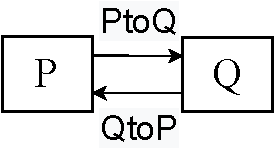
\includegraphics[scale=0.4]{figures/p_and_q.pdf}
	\caption{$P$ and $Q$ connected by two logical channels which are actually implemented by the figure on the right.}
	\label{fig:pandq}
	\end{subfigure}
	\\
	\begin{subfigure}{0.5\textwidth}
	\centering
	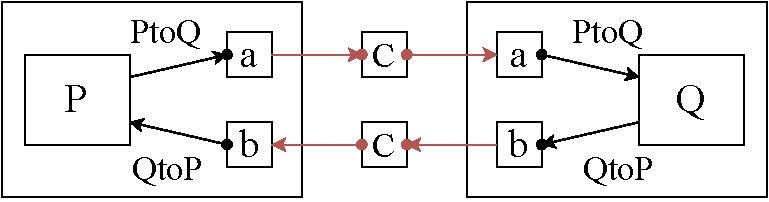
\includegraphics[scale=0.4]{figures/new_p_and_q.pdf}
	\caption{We can realize the left be intermediating communication with communicators. The direction of messages from $P$ to $Q$ still suggest a cycle but the communicator is provider (dot) to \emph{both} shell codes.}
	\label{fig:newpandq}
	\end{subfigure}
	\caption{Two ITM configurations. One possible with ITMs (left) and one realized in NomosUC (right). Arrows indicate direction of messages and the dot indicates the provider of the channel.}
	\vspace{-5mm}
\end{figure}

In general, we represent communication between any two ITMs as two providerless channels.
We further don't restrict the types of the two channels, and allow them to each be bidirectional as well.
However, for simplicity, and to be as generalized as possible, we stick to two uni-directonal channels as that directly resolves the internal vs external choice that arises from a single session type capturing $P$ and $Q$.

